En esta sección se presentan las ejecuciones realizadas con Apache Pig y HCatalog para el objetivo específico 3 del presente proyecto. \\

\subsection{Problemas tratados}

\subsubsection{Problema 1:} Determinar la temperatura promedio registrada por año para los años mayores a 1950, teniendo como base los datos consignados en el dataset del NCDC.

\subsubsection{Problema 2:} Determinar la temperatura promedio registrada para el año 1910, teniendo como base los datos consignados en el dataset del NCDC.

\subsection{Estrategia problema 2: Apache Pig y HCatalog}

A continuación se detallan los pasos necesarios para resolver el problema 2, usando Pig y HCatalog. \\

\subsubsection{Definición del script en PigLatin}

El siguiente script contiene el código utilizado utilizado para ejecutar el programa \textit{AverageTemperature} en PigLatin. En las primera lineas del script se detalla el uso de una UDF (\textit{User defined function}), provista por Tom White, para minimizar el código necesario en el filtrado de registros. En la segunda línea se define el uso de HCatalog para el acceso al \textit{metastore} de Hive. El contenido del script fue guardado en un archivo llamado \textit{avg-1910-temp-hcatalog.pig}.

\begin{lstlisting}[linewidth=\columnwidth,breaklines=true]
REGISTER $load_loc;
records = LOAD '$table_name' USING &org.apache.hive.hcatalog.pig.HCatLoader()&;
filtered_records = FILTER records BY air_temperature != 9999 AND &com.hadoopbook.pig.IsGoodQuality&((int)at_quality_code) AND observation_date_year == 1910; 
grouped_records = GROUP filtered_records BY observation_date_year; 
avg_temp = FOREACH grouped_records GENERATE group,AVG(filtered_records.air_temperature); 
DUMP avg_temp;  
\end{lstlisting} 


\subsubsection{Definición de los parámetros del script}

Una vez definido el script en PigLatin, se procede a definir en un nuevo archivo los parámetros necesarios para la correcta ejecución del script. Los parámetros mencionados fueron guardados en un archivo llamado \textit{avg-1910-hcatalog-managed-pb.param}.

\begin{lstlisting}[linewidth=\columnwidth,breaklines=true]
# Load function location.
load_loc=/home/sas6/Oozie-Pig-HCatalog-Demos/assets/&pig&-examples.jar
# Input.
table_name=weather_managed_pb
\end{lstlisting}

\subsubsection{Ejecución con Grunt en modo \textit{batch}}

A continuación se detalla el comando utilizado para ejecutar el programa \textit{AverageTemperature} mediante el modo \textit{batch} de Grunt.

\begin{lstlisting}[linewidth=\columnwidth,breaklines=true]
pig -param_file /home/sas6/Oozie-Pig-HCatalog-Demos/scripts/&pig&/300GB/avg_1910_hcatalog_managed_pb.param /home/sas6/Oozie-Pig-HCatalog-Demos/src/&pig&/avg-1910-temp-hcatalog.&pig&
\end{lstlisting}

\subsubsection{Seguimiento a la ejecución del programa}

El monitoreo de la ejecución del programa podrá realizarse a través de Grunt, por medio de la interfaz gráfica de YARN, o por la información proporcionada por el Job History Server.

\begin{figure}[H]
  \centering
      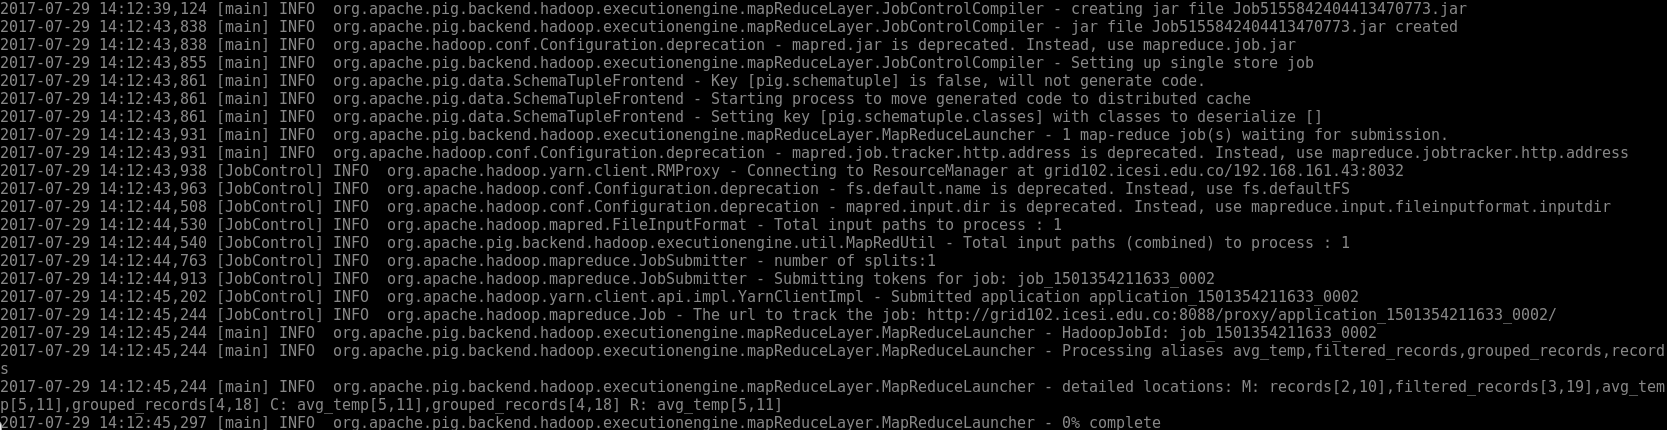
\includegraphics[width=\textwidth, height=2.0in]{fig/05/04}
  \caption{Monitoreo de la ejecución del programa \textit{AverageTemperature} en Pig por medio de la consola Grunt desde donde se ejecutó.}
\end{figure}

\begin{figure}[H]
  \centering
      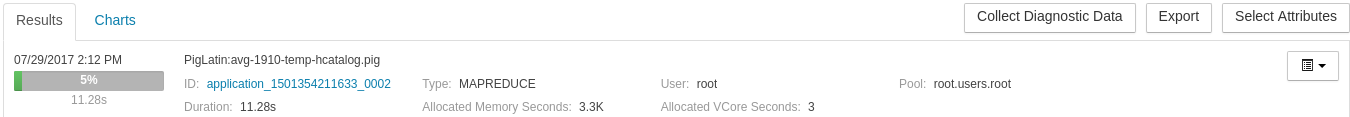
\includegraphics[width=\textwidth, height=0.8in]{fig/05/05}
  \caption{Monitoreo de la ejecución del programa \textit{AverageTemperature} en Pig por medio de la interfaz de YARN.}
\end{figure}

\begin{figure}[H]
  \centering
      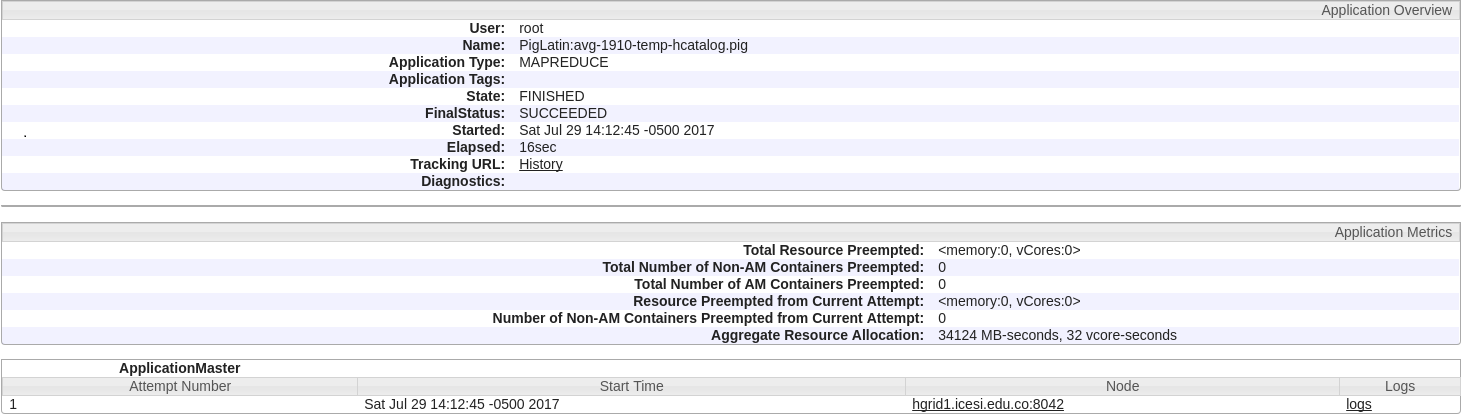
\includegraphics[width=\textwidth, height=2.7in]{fig/05/06}
  \caption{Ejecución finalizada, vista desde el Job History Server.}
\end{figure}